In this lab we will use Paraben's E3 tool to load and sort digital evidence to view suspicious chats and email messages.

\section*{Part 1: Create and Sort a New Case File}
\begin{figure}[H]
    \centering
    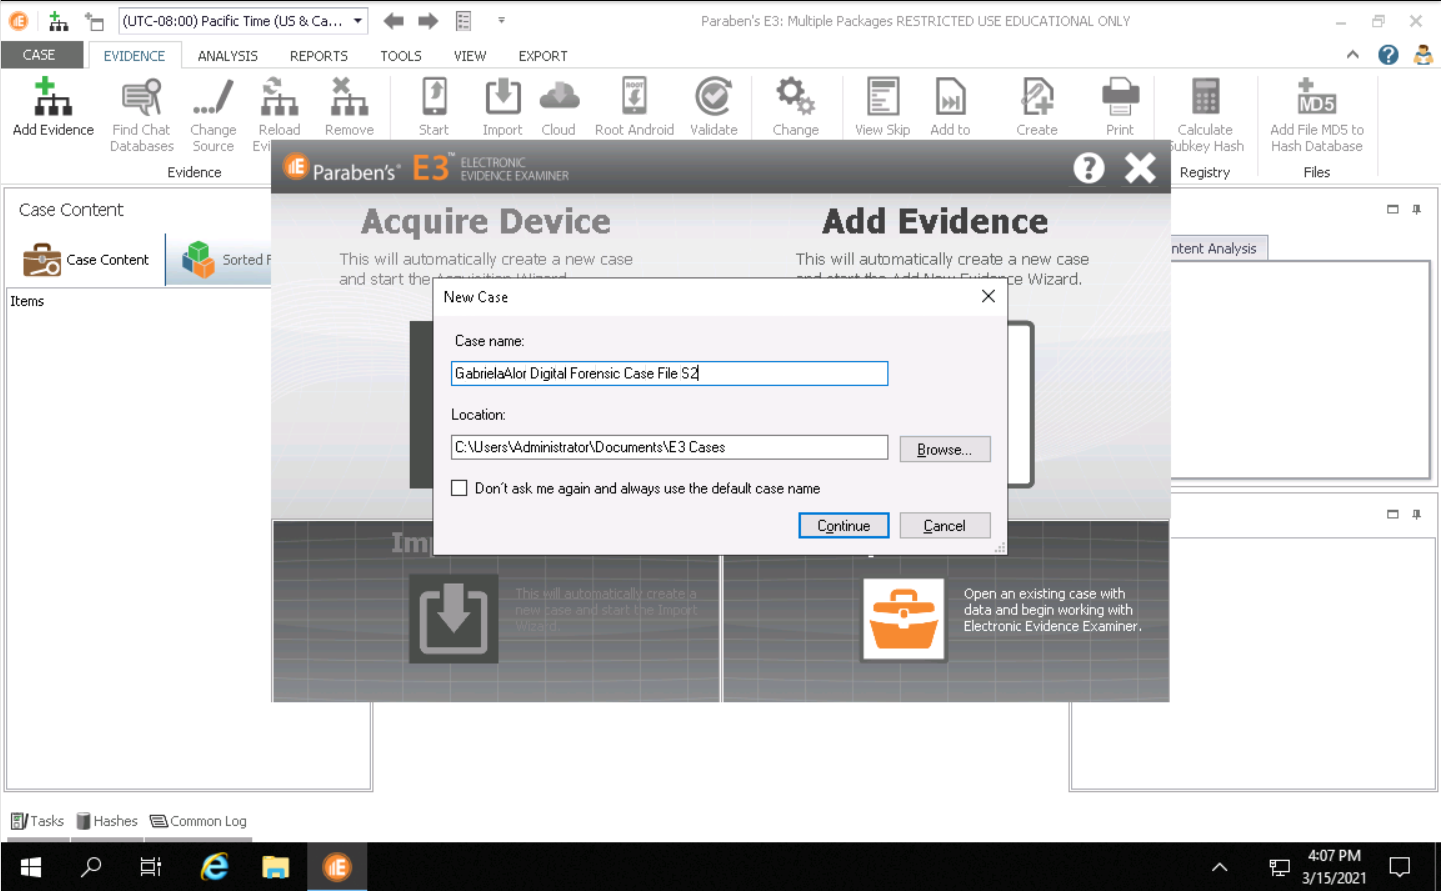
\includegraphics[width=\linewidth]{figures/1-2.png}
    \caption{Creation of evidence file.}
\end{figure}

\begin{figure}[H]
    \centering
    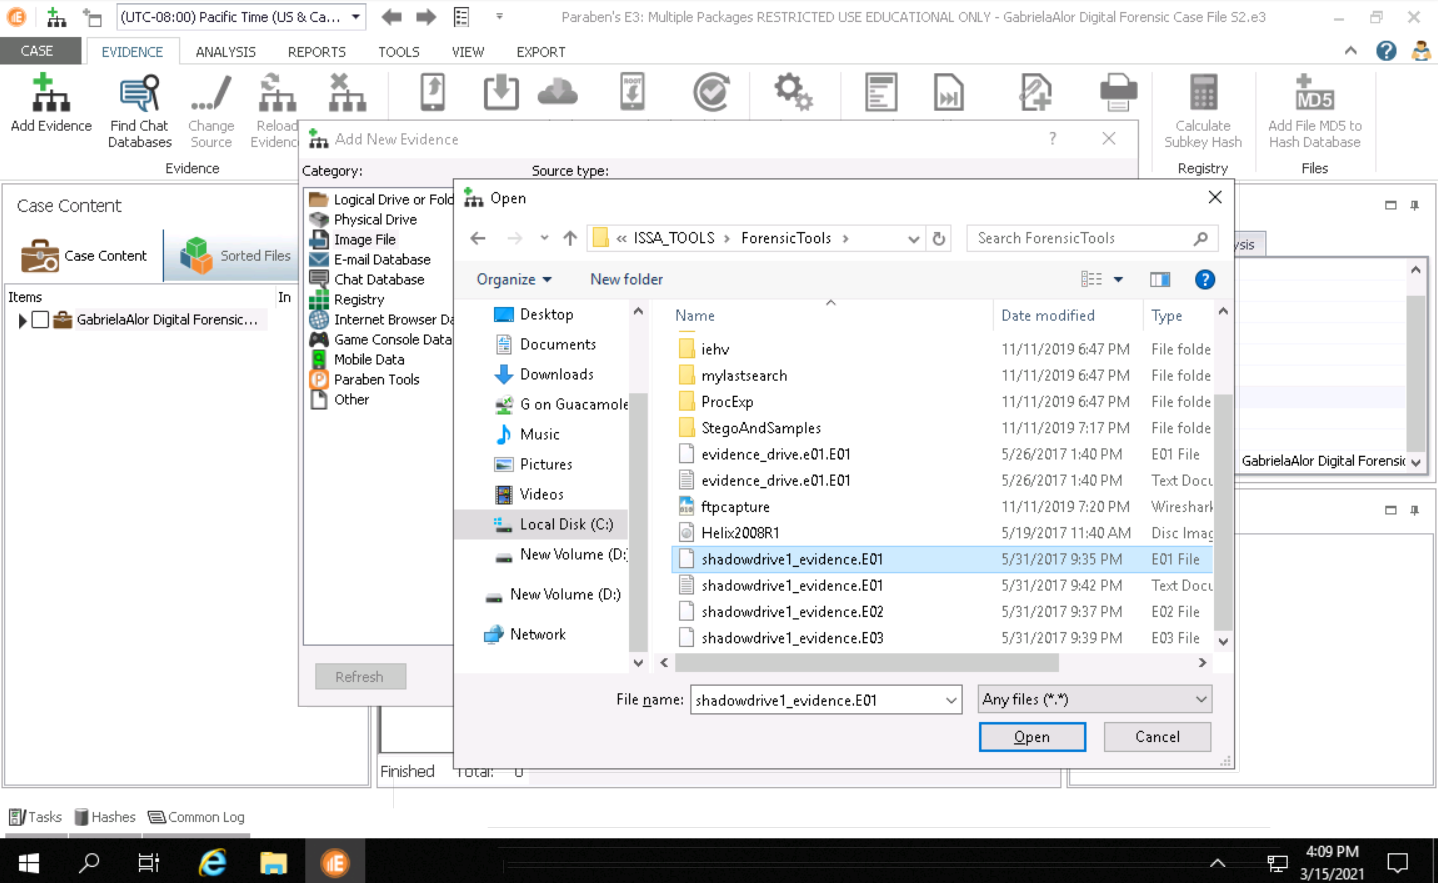
\includegraphics[width=\linewidth]{figures/1-3.png}
    \caption{Adding digital drive image to the evidence file.}
\end{figure}

\begin{figure}[H]
    \centering
    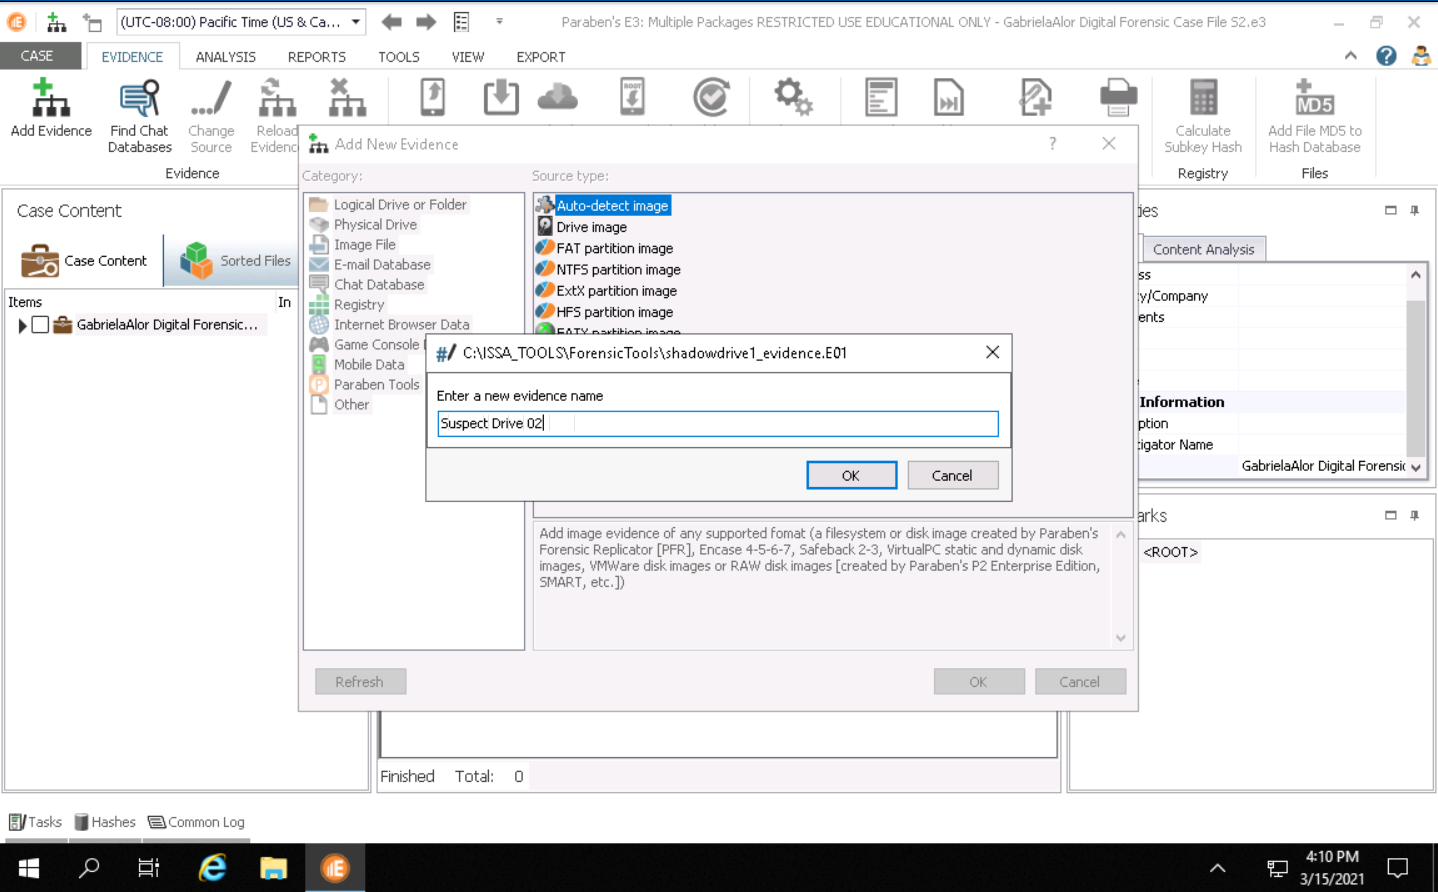
\includegraphics[width=\linewidth]{figures/1-4.png}
    \caption{Naming the evidence drive.}
\end{figure}

\begin{figure}[H]
    \centering
    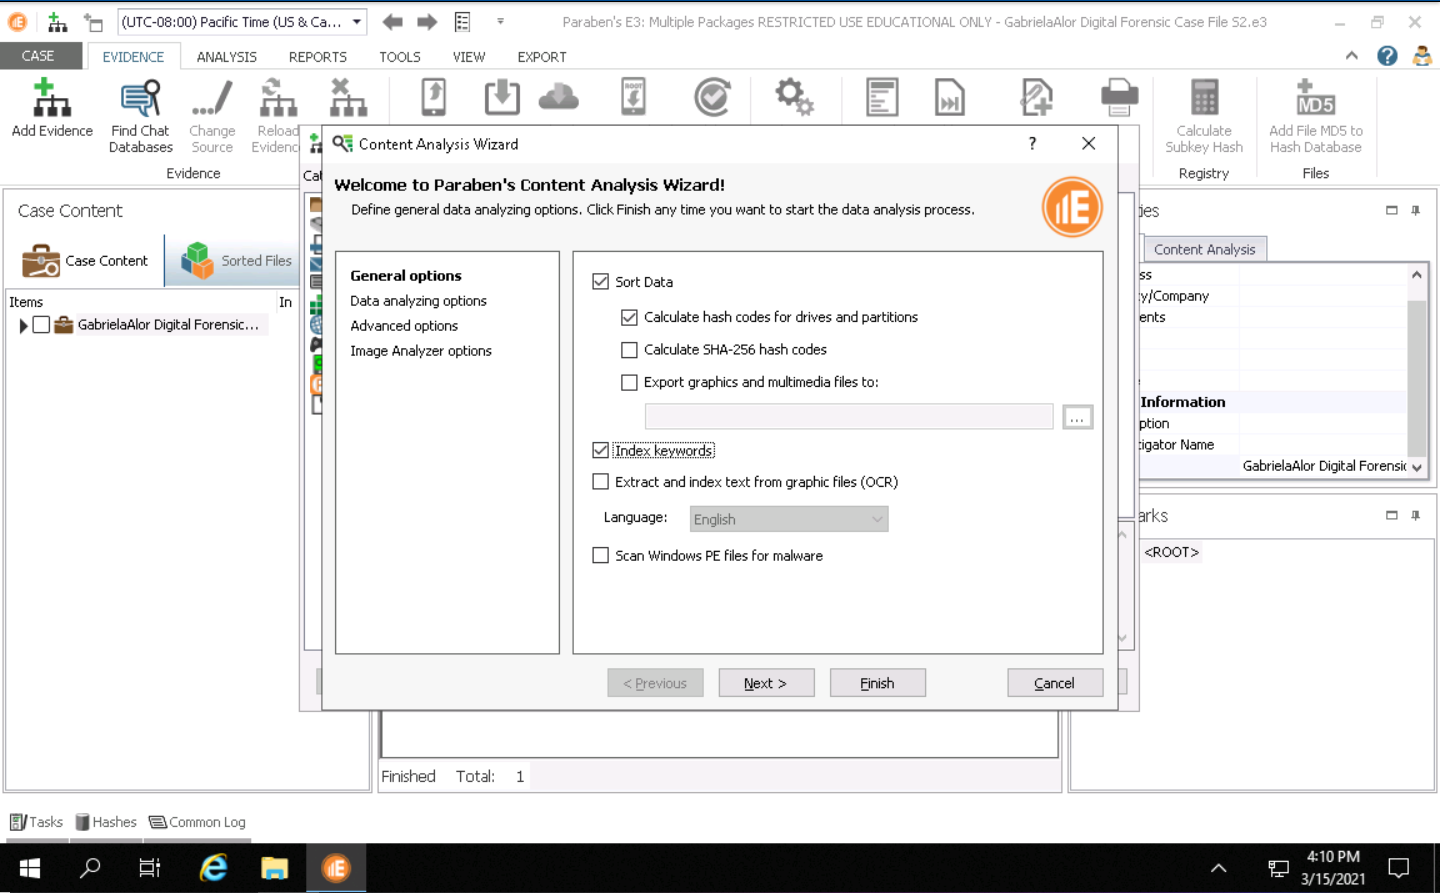
\includegraphics[width=\linewidth]{figures/1-5.png}
    \caption{Calculating hash codes for drives and partitions.}
\end{figure}

\begin{figure}[H]
    \centering
    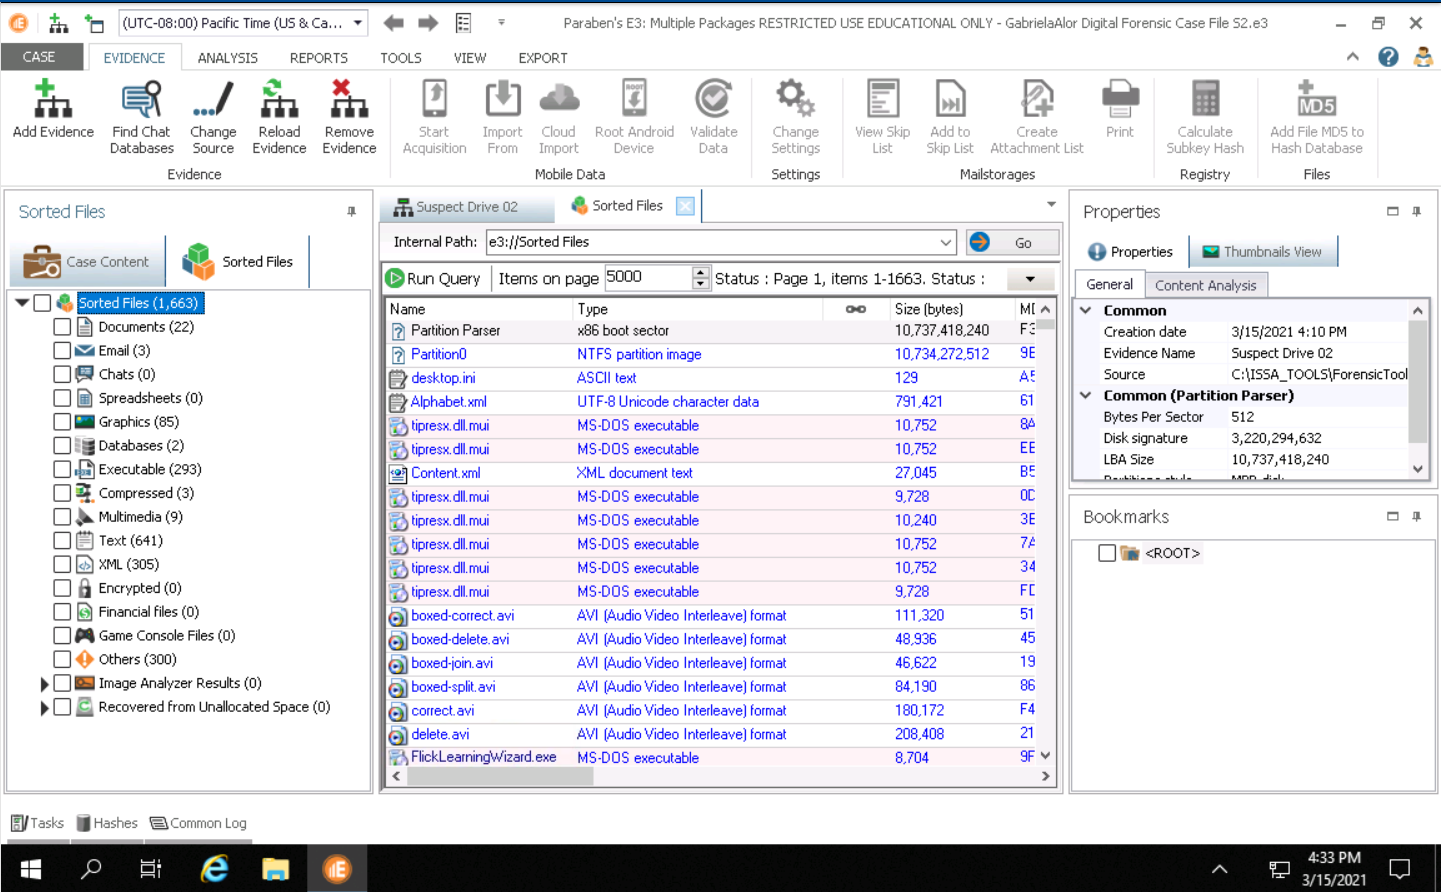
\includegraphics[width=\linewidth]{figures/1-8.png}
    \caption{Sorted evidence.}
\end{figure}

\section*{Part 2: Explore Chat and E-mail Conversations}
\begin{figure}[H]
    \centering
    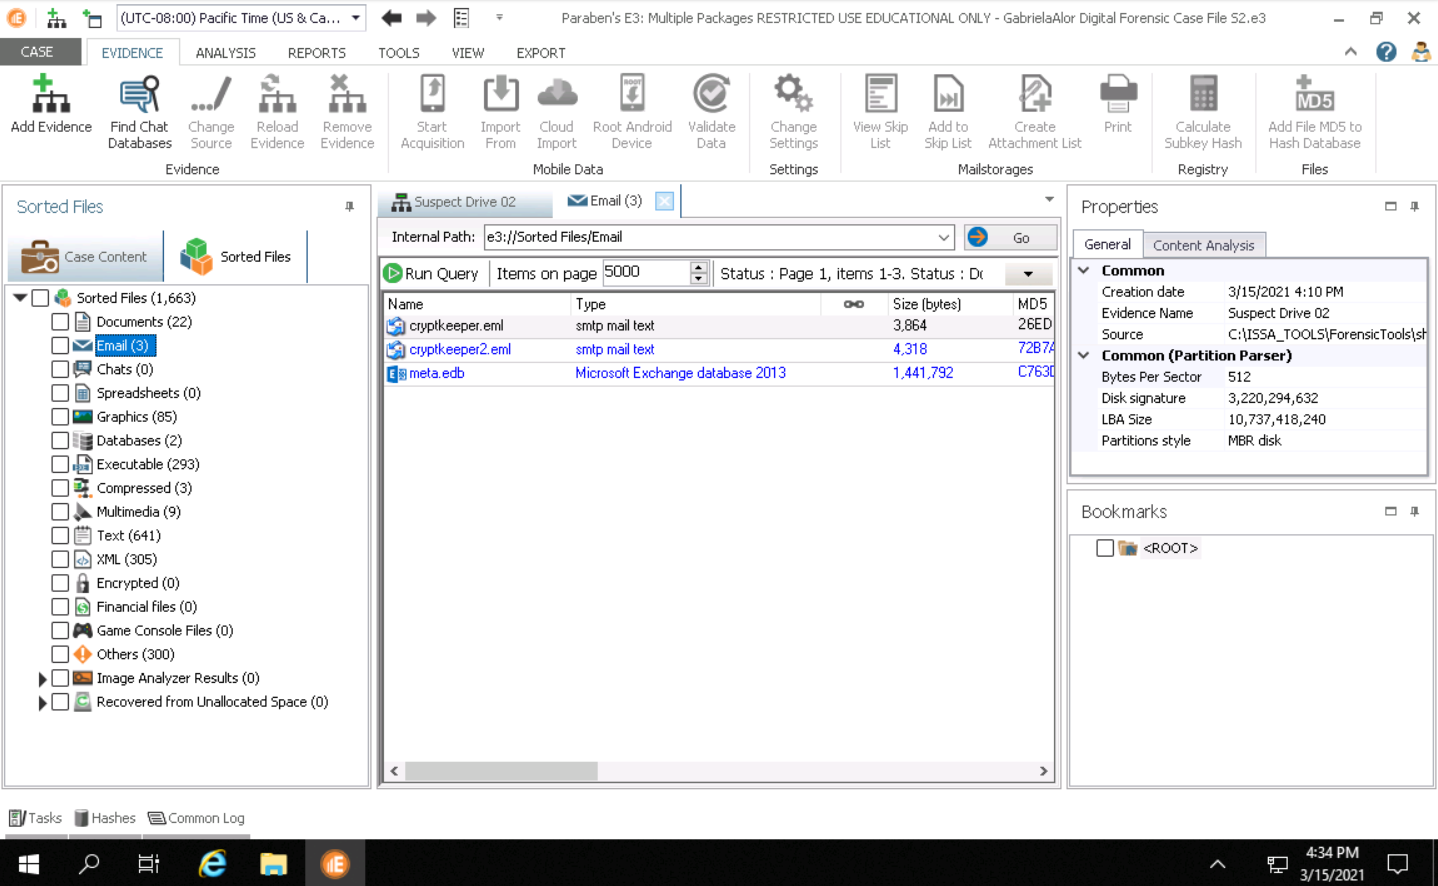
\includegraphics[width=\linewidth]{figures/2-1.png}
    \caption{Email evidence category.}
\end{figure}

\begin{figure}[H]
    \centering
    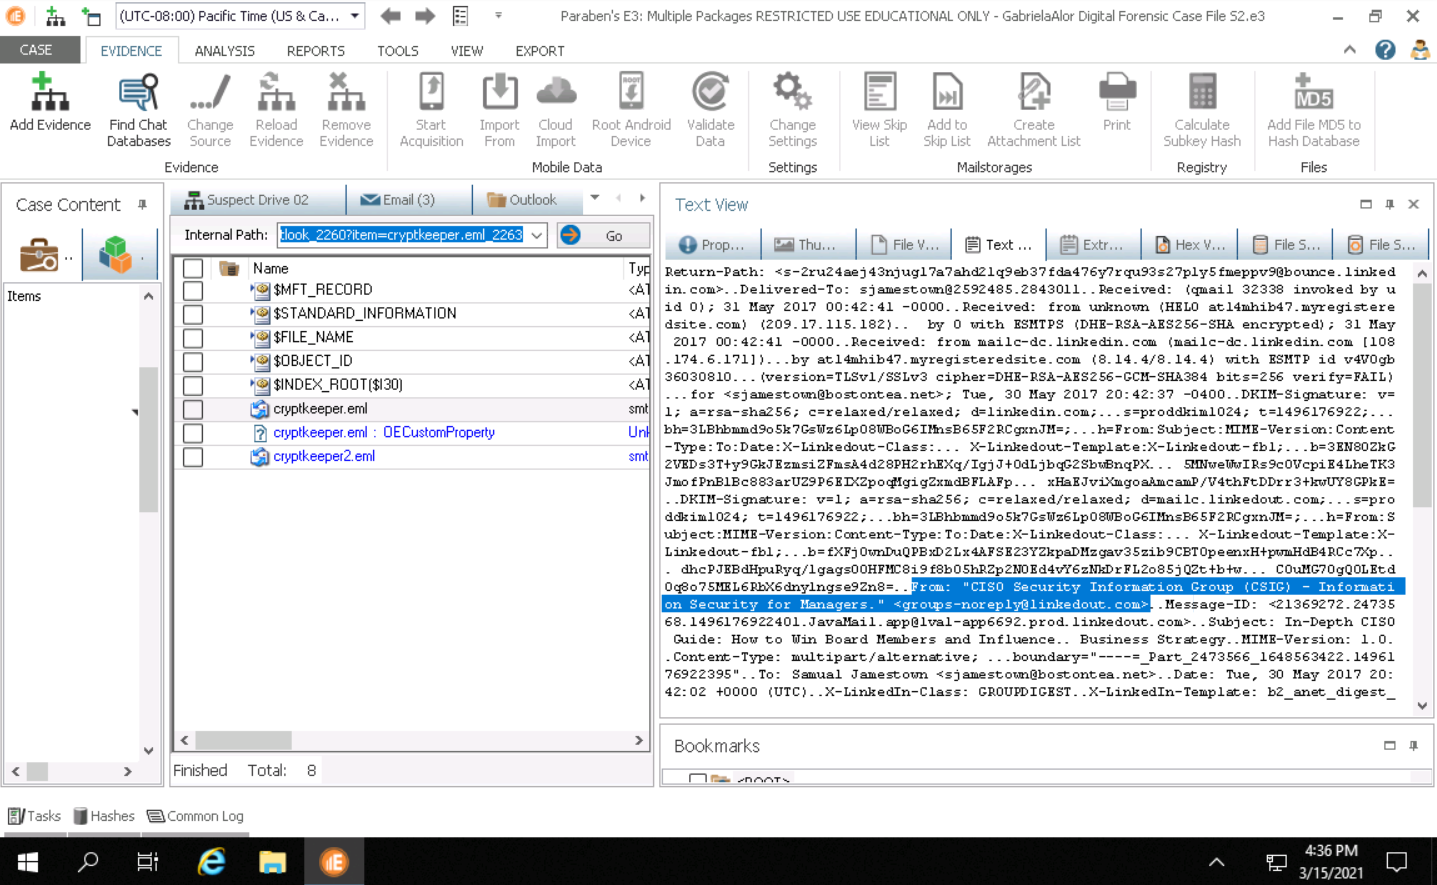
\includegraphics[width=\linewidth]{figures/2-6.png}
    \caption{Contents of cryptkeeper.eml evidence.}
\end{figure}

\begin{figure}[H]
    \centering
    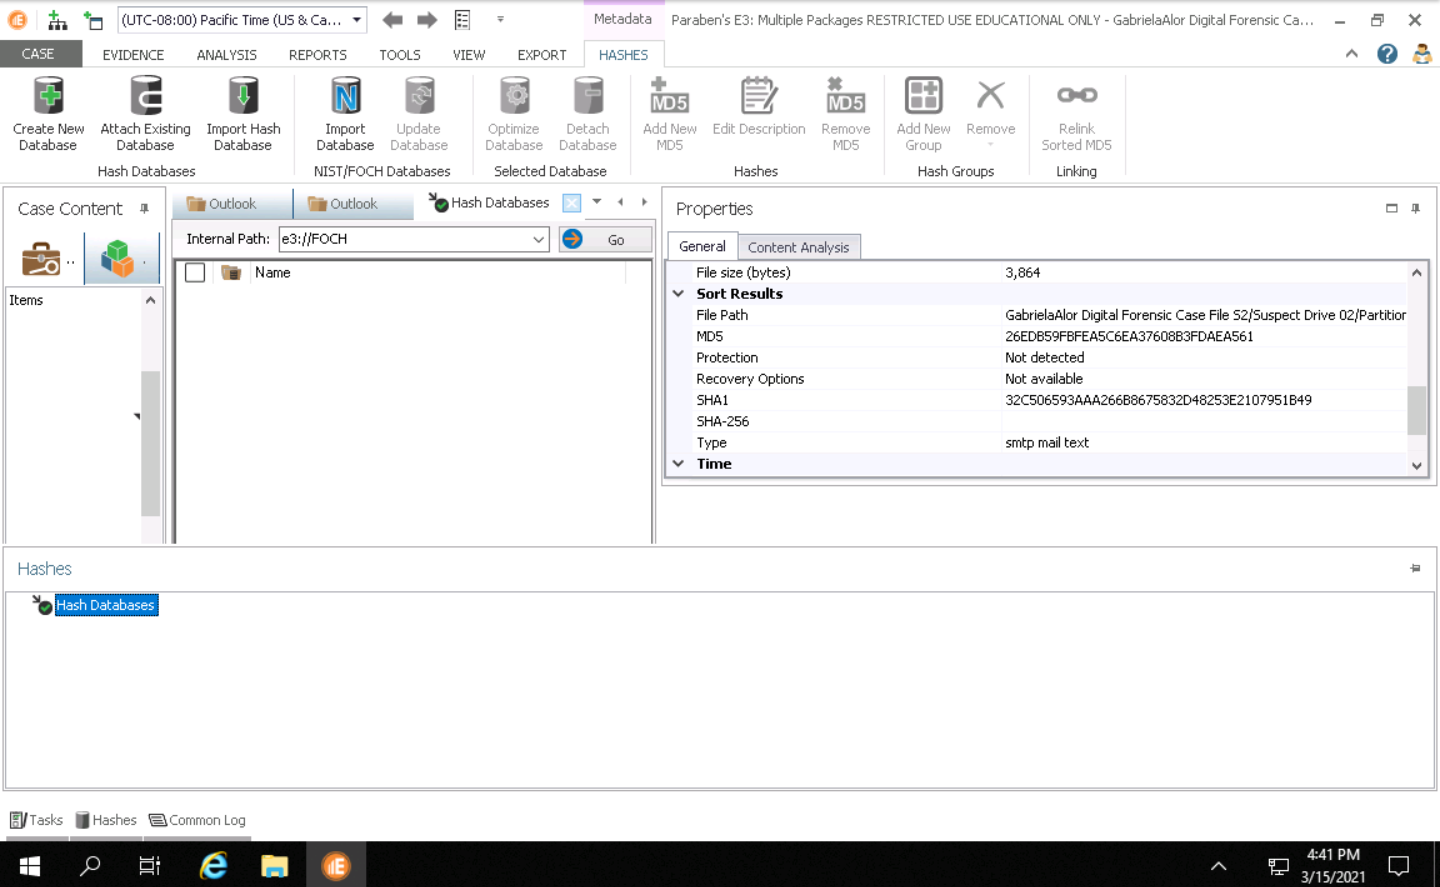
\includegraphics[width=\linewidth]{figures/2-7.png}
    \caption{MD5 and SHA1 hashes for cryptkeeper.eml}
\end{figure}

\begin{figure}[H]
    \centering
    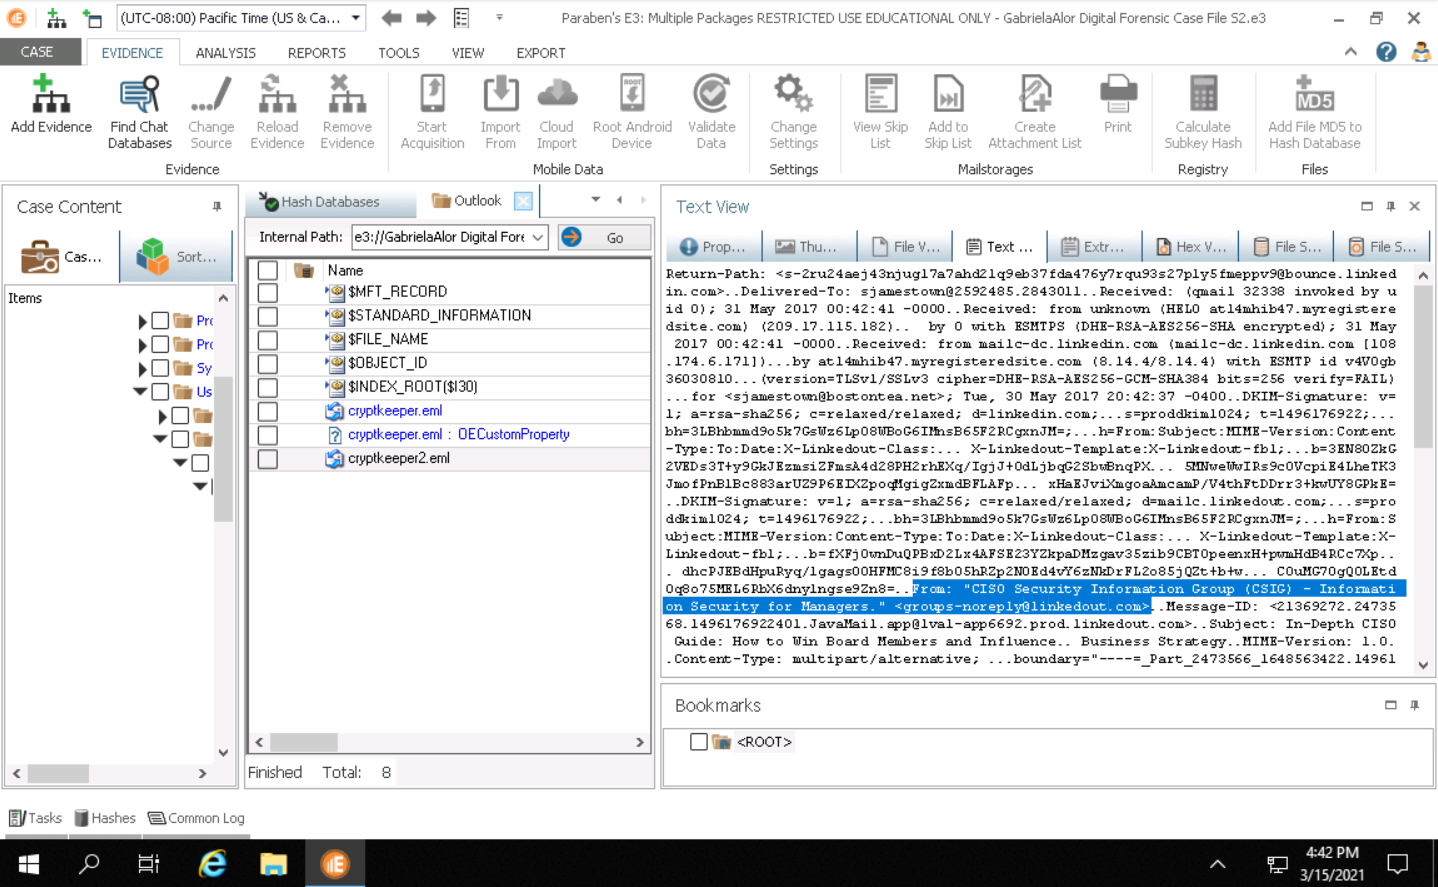
\includegraphics[width=\linewidth]{figures/2-10.png}
    \caption{Contents of cryptkeeper2.eml evidence.}
\end{figure}

\begin{figure}[H]
    \centering
    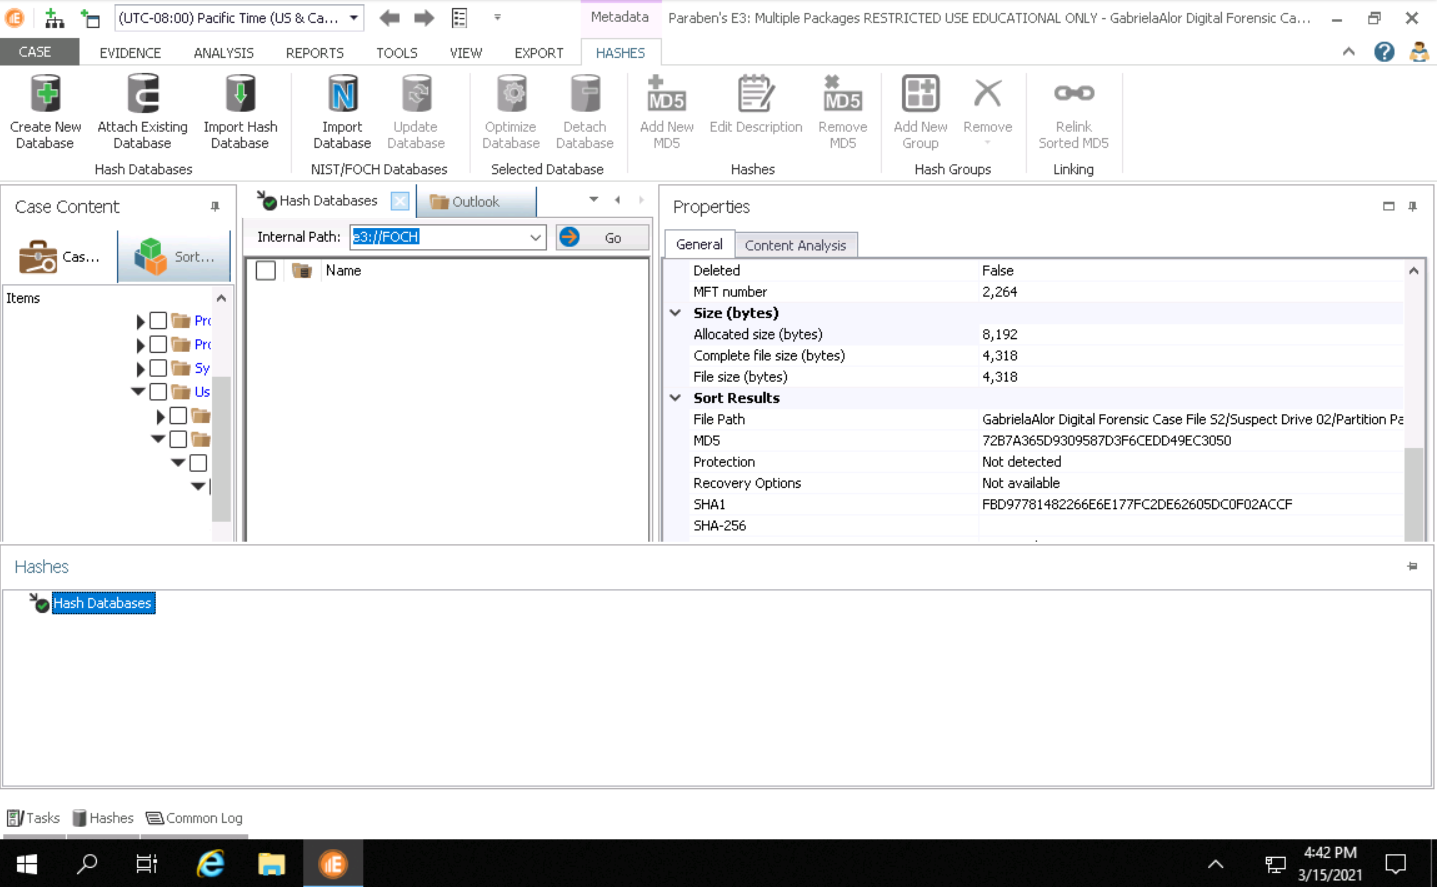
\includegraphics[width=\linewidth]{figures/2-11.png}
    \caption{MD5 and SHA1 values for cryptkeeper2.eml evidence file.}
\end{figure}

\begin{figure}[H]
    \centering
    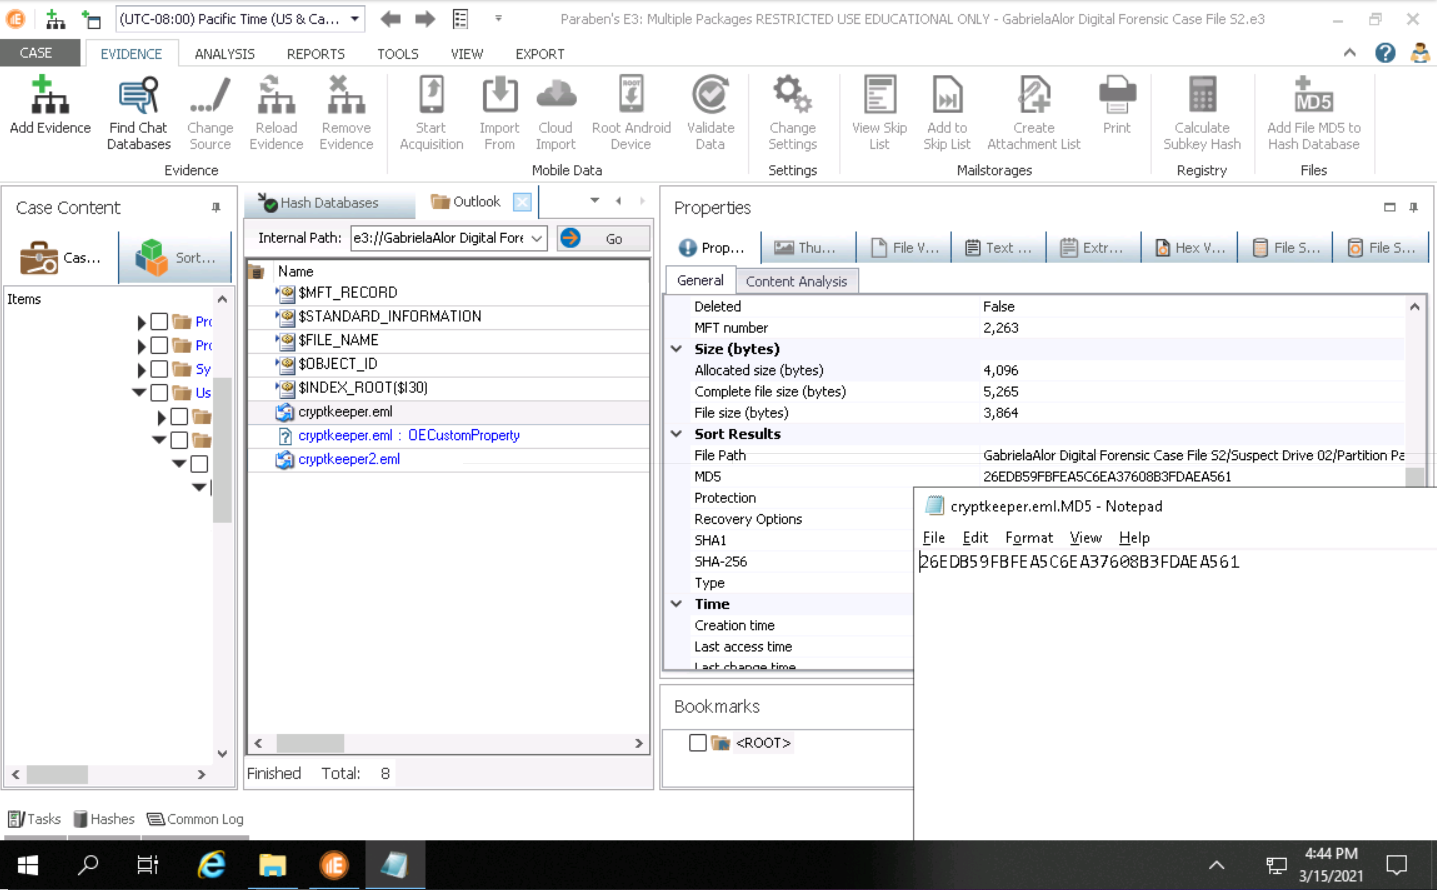
\includegraphics[width=\linewidth]{figures/2-12.png}
    \caption{Comparison of cryptkeeper.eml MD5 values from step 7.}
\end{figure}

\begin{figure}[H]
    \centering
    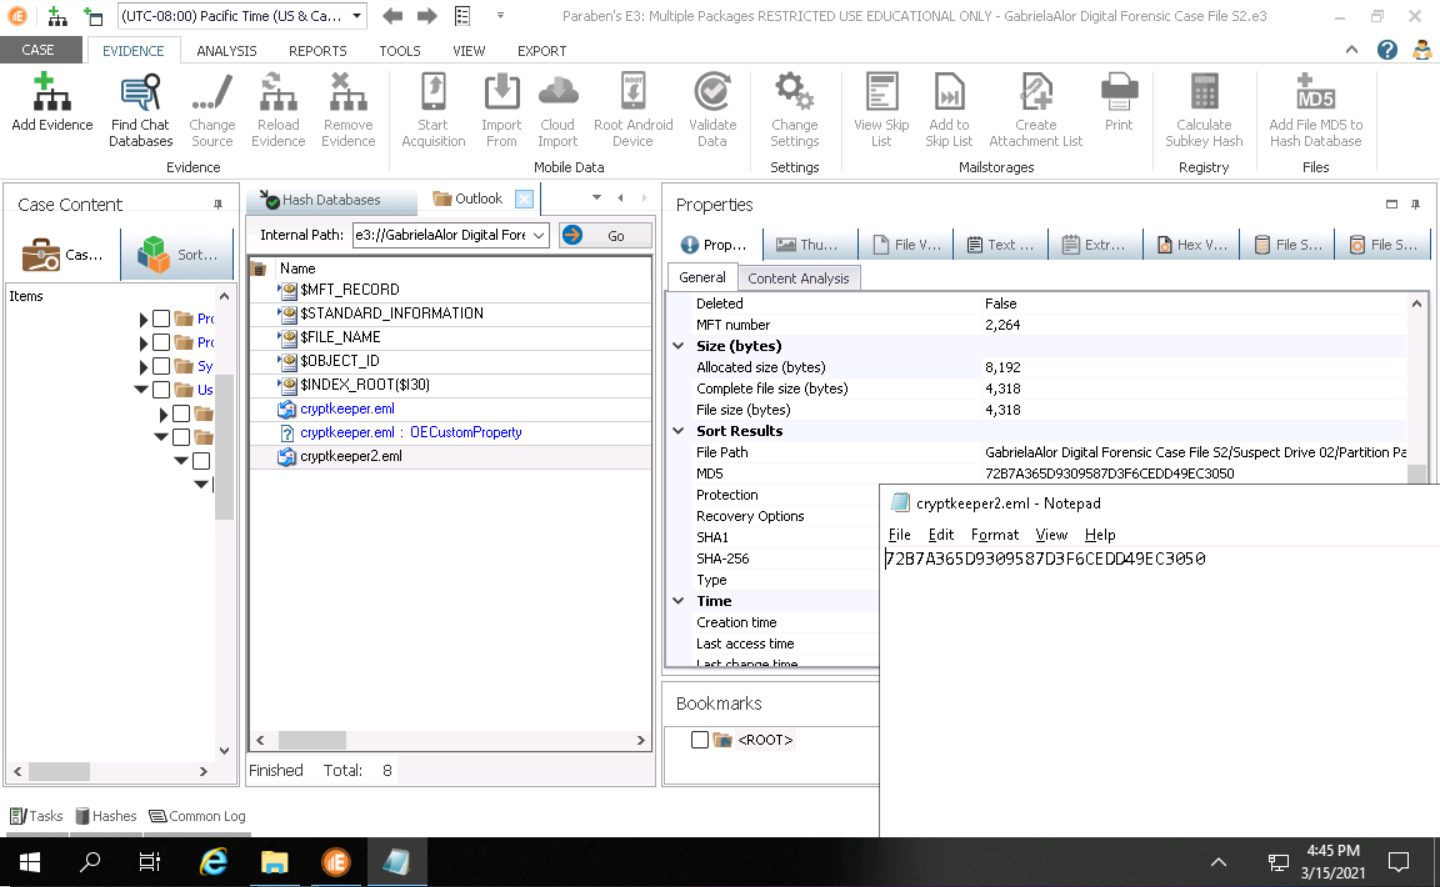
\includegraphics[width=\linewidth]{figures/2-13.png}
    \caption{Comparison of cryptkeeper2.eml MD5 hash values from step 7.}
\end{figure}

\begin{figure}[H]
    \centering
    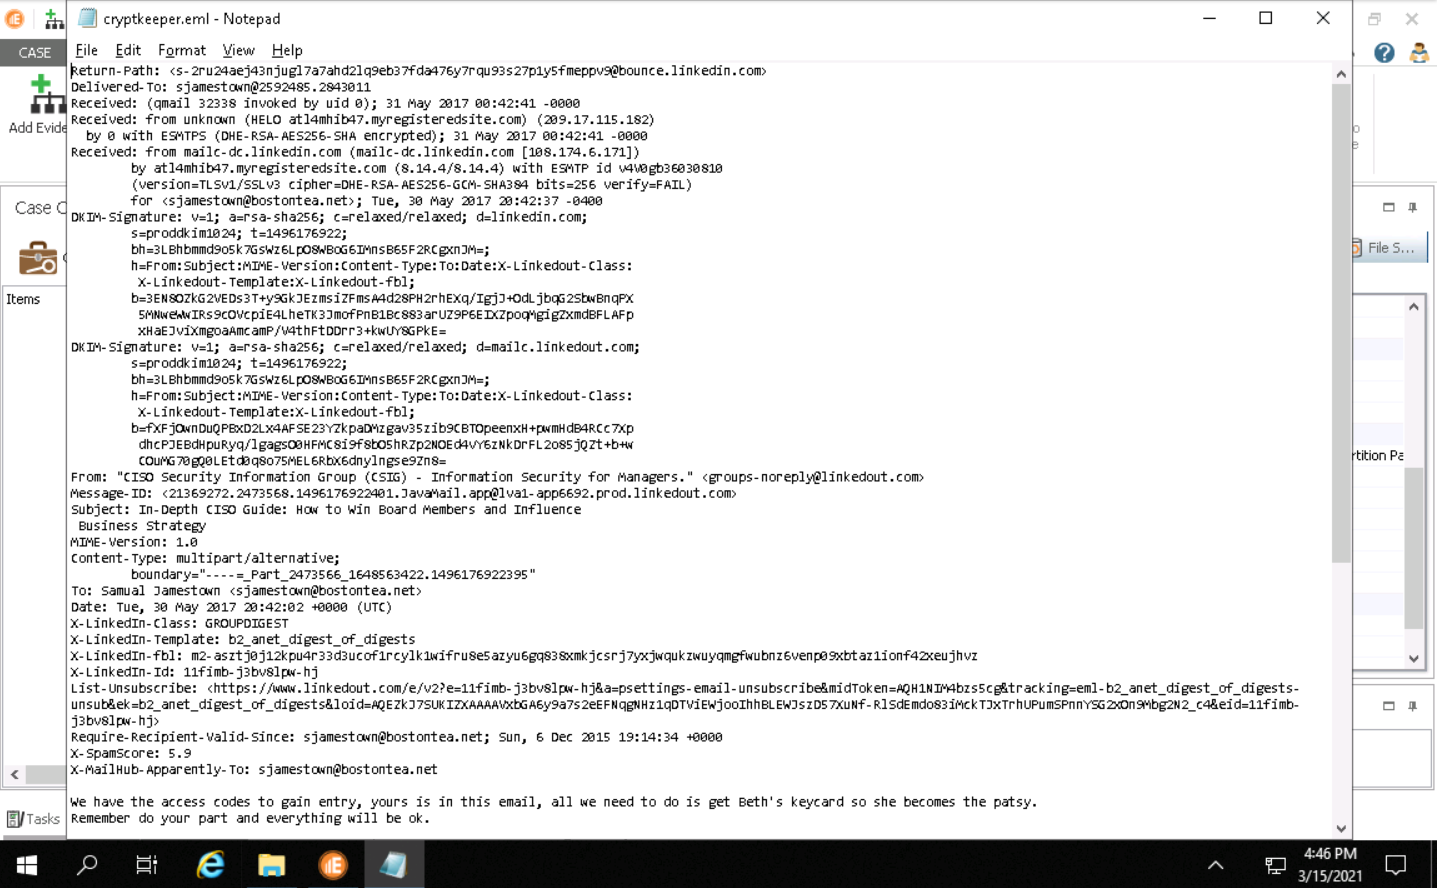
\includegraphics[width=\linewidth]{figures/2-14.png}
    \caption{Contents of cryptkeeper.eml.}
\end{figure}

\begin{figure}[H]
    \centering
    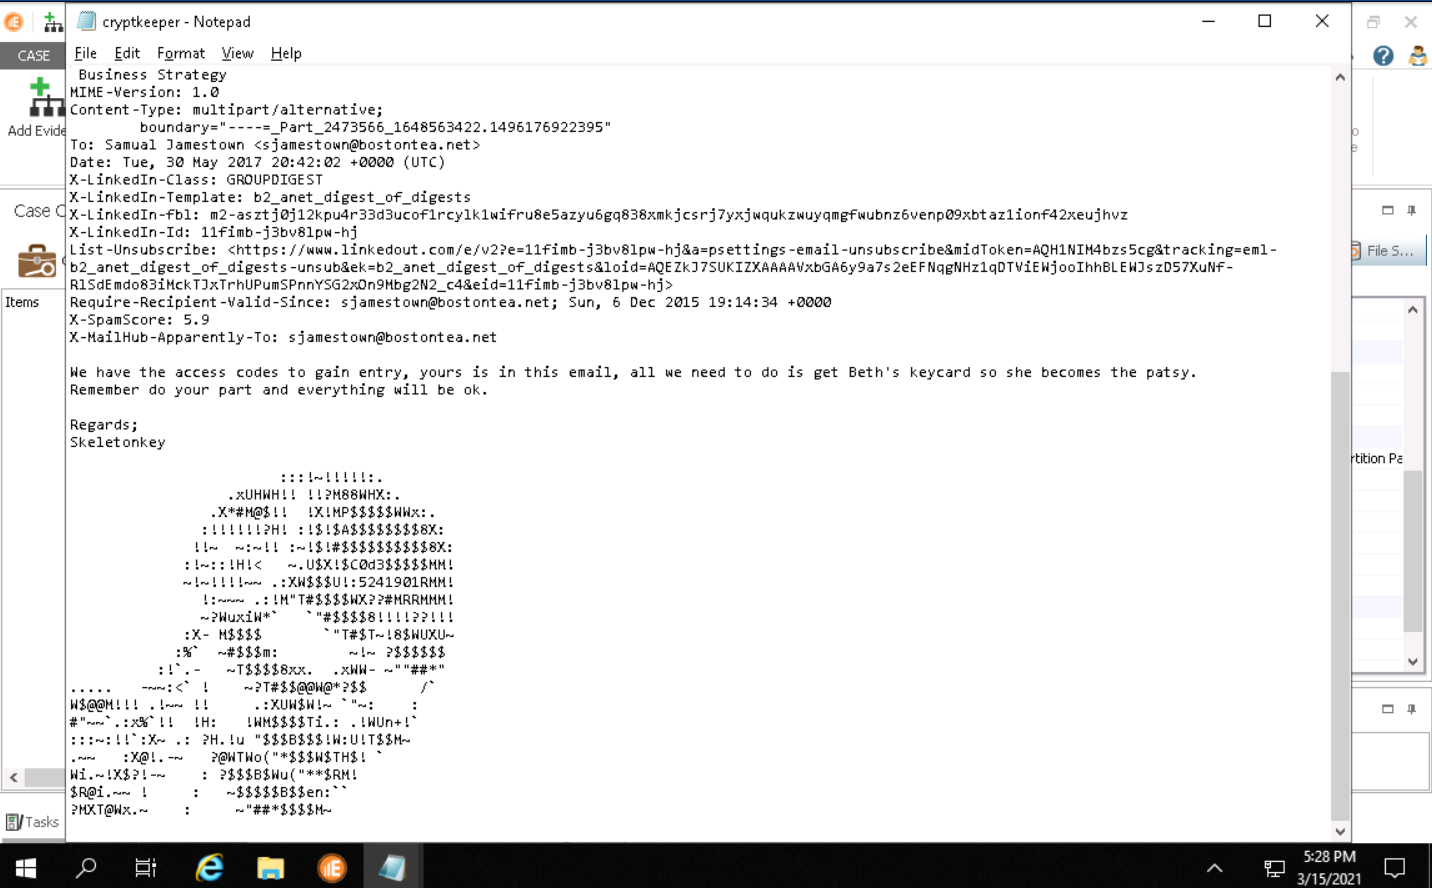
\includegraphics[width=\linewidth]{figures/2-15.png}
    \caption{Contents of cryptkeeper.eml continued.}
\end{figure}

\begin{figure}[H]
    \centering
    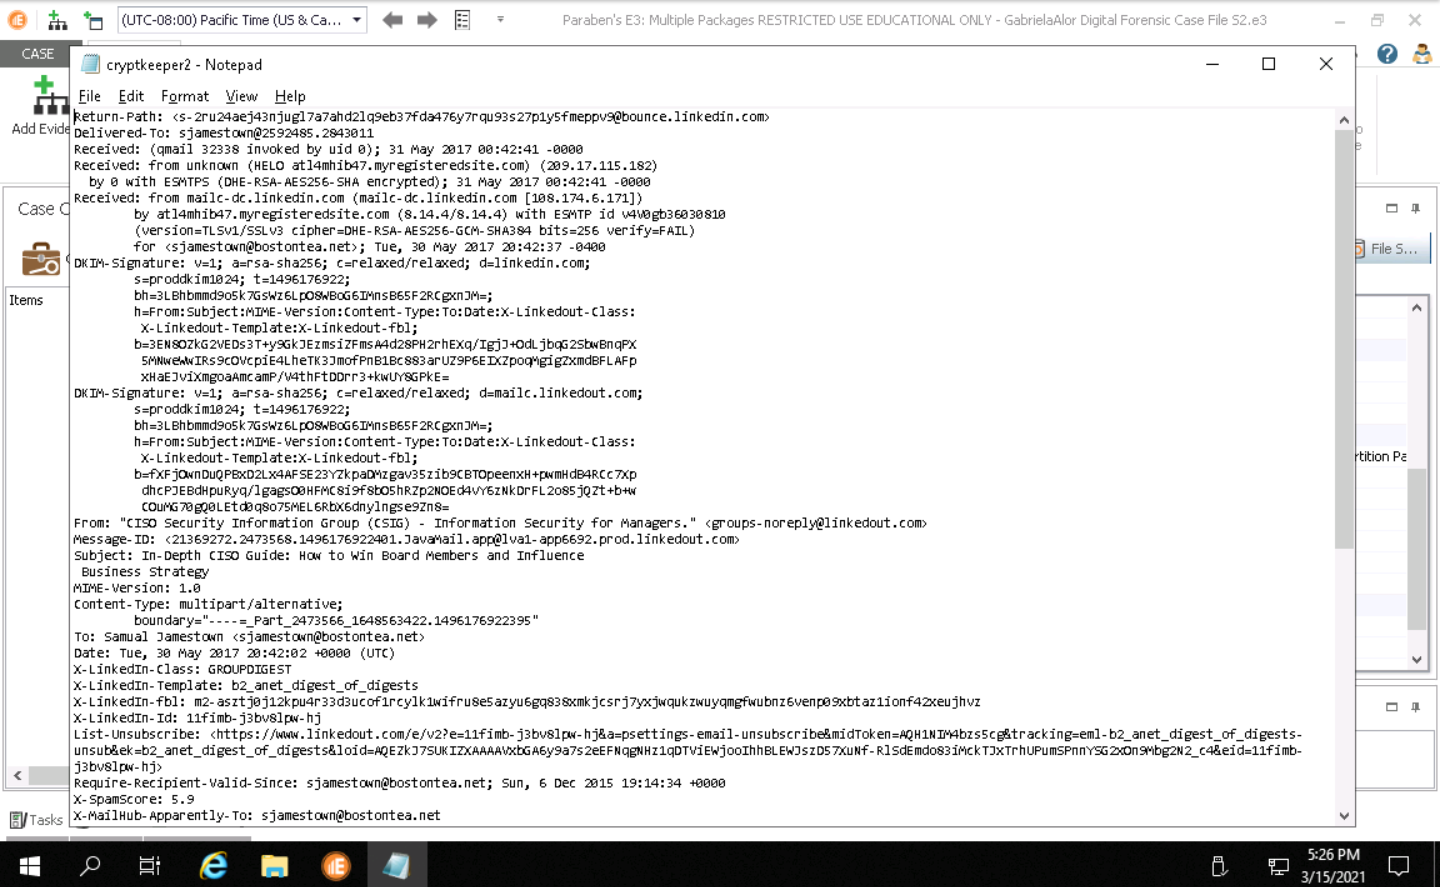
\includegraphics[width=\linewidth]{figures/2-16.png}
    \caption{Contents of cryptkeeper2.eml.}
\end{figure}

\begin{figure}[H]
    \centering
    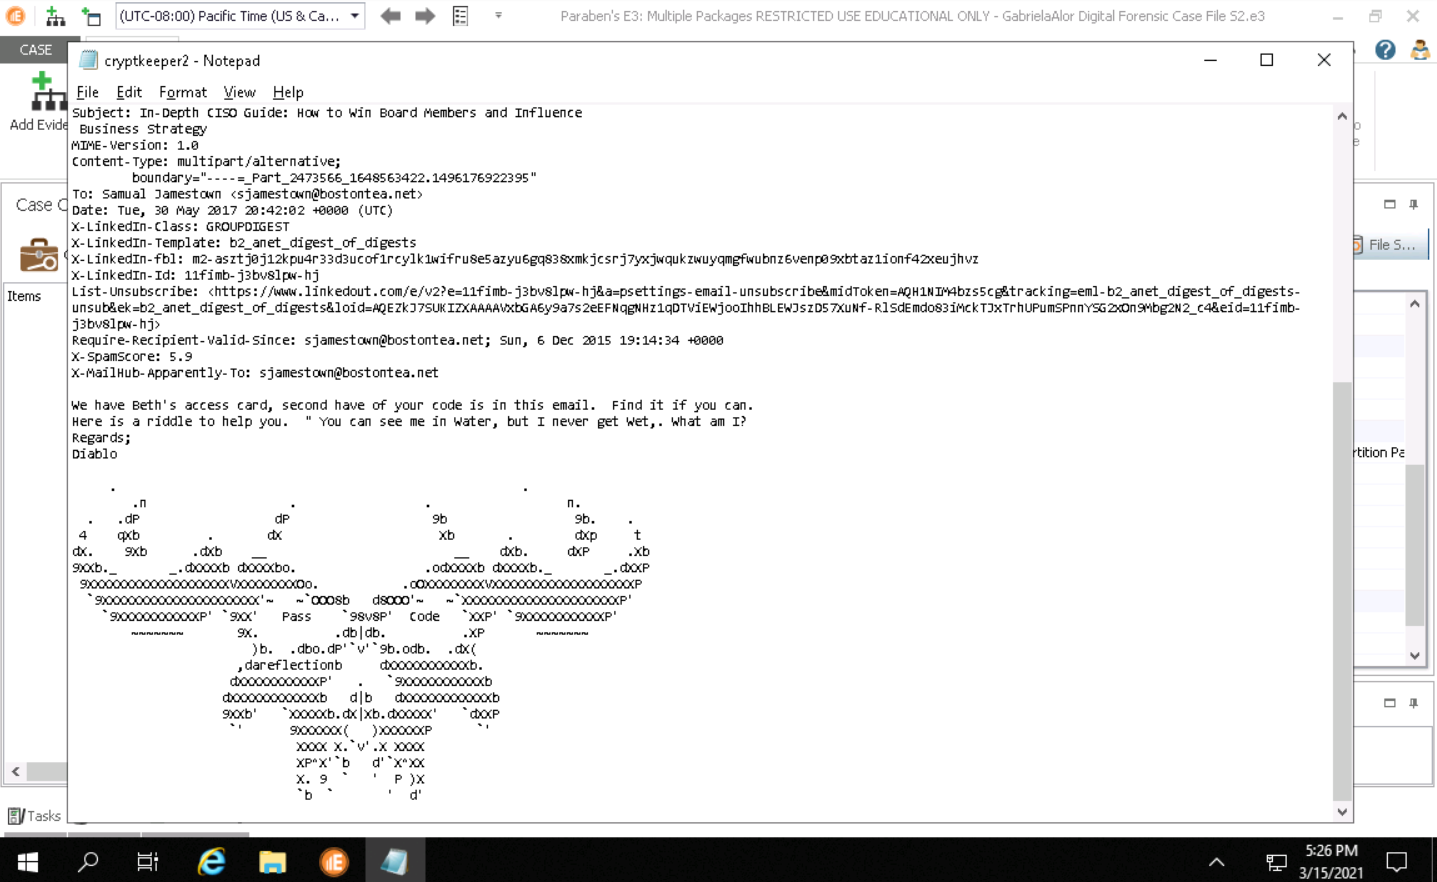
\includegraphics[width=\linewidth]{figures/2-17.png}
    \caption{Contents of cryptkeeper2.eml continued.}
\end{figure}

In this lab we learned how to use Paraben's E3 evidence tool to view email evidence.
The tool allows us to view metadata for the email, showing creation dates.
We were able to observe the contents of the email as well.
Calculating the hashes of files is done with the hash tool.
This allows us to determine if any evidence was altered during the examination process.